\documentclass[graphics]{beamer}
\usepackage{graphicx}
\usepackage{listings} % Syntax highlighing
\usepackage{fancyvrb} % Inline verbatim
\hypersetup{bookmarksopen=true,bookmarksopenlevel=4,pdfdisplaydoctitle=true,pdfpagemode=FullScreen}

\usepackage[normalem]{ulem}               % to strikethrough text
\newcommand\redout{\bgroup\markoverwith
{\textcolor{red}{\rule[0.5ex]{2pt}{0.8pt}}}\ULon}

% header in tables
\newcommand*{\thead}[1]{\multicolumn{1}{c}{\bfseries #1}}

% used for arrows from one point in the slide to another
\usepackage{tikz}
\usetikzlibrary{arrows,shapes,tikzmark}

\usetheme{Boadilla}
\title{Lecture 2: Architecture \& Number Systems}
\author{UMBC CMSC 104}
\date{Tu 6 Sept 2022}

\begin{document}

\begin{frame}{}
\centering
    Machine Architecture and Number Systems
\end{frame}

\frame{\tableofcontents}

\begin{frame}{Why are we in this course?}
    \only<1> {
        \center{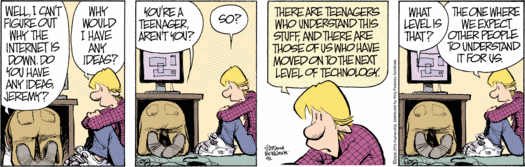
\includegraphics[scale=0.61]{L02_ArchNumbersSystems/L2_p2.png}}
        
        \newline
        Remember: ``There are no stupid questions, just stupid people who don't know they should be asking something''
    }
    \only<2> {
        \begin{itemize}
            \item Technology is everywhere: phones, computers, tablets, game consoles, etc.
            \item It's important to understand that which we all rely on for important activities.
            \item To understand what technology is and how it works is to be better empowered to make decisions.
            \item ``Program, or be programmed''\footnote{\url{https://www.opensourcevoices.org/24}}: Learn how technology works, and use it as you wish; or only use technology in the manner that you're told to do so by big companies.
        \end{itemize}
    }
\end{frame}

%\begin{frame}{Machine Architecture \& Number Systems}
%Topics:
%\begin{itemize}
%    \item Major computer components
%    \item Bits, bytes, words
%    \item The Decimal number system
%    \item The Binary number system
%    \item Converting from Binary to Decimal
%    \item Converting from Decimal to Binary
%    \item The Hexadecimal number system
%\end{itemize}
%\end{frame}

\section{Computer Examples}
\begin{frame}{Some People Think a Computer is...}
    \centering
    \only<1>{
        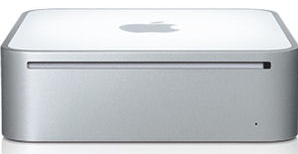
\includegraphics[scale=0.8]{L02_ArchNumbersSystems/L2_p4.png}
    }
    \only<2>{
        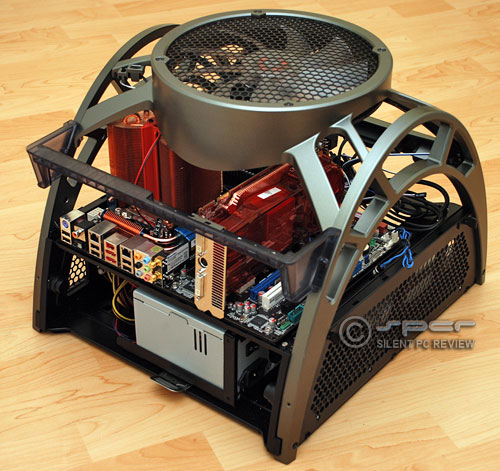
\includegraphics[scale=0.65]{L02_ArchNumbersSystems/L2_p5.png}
    }
\end{frame}

\begin{frame}{Extreme Examples}
    \begin{columns}
        \column{0.4\textwidth}
            \includegraphics[scale=0.1]{L02_ArchNumbersSystems/L2_rasppi.jpg}
            Raspberry Pi \$35 computer
            \footnotesize
            \url{https://www.raspberrypi.org/}
        \column{0.6\textwidth}
            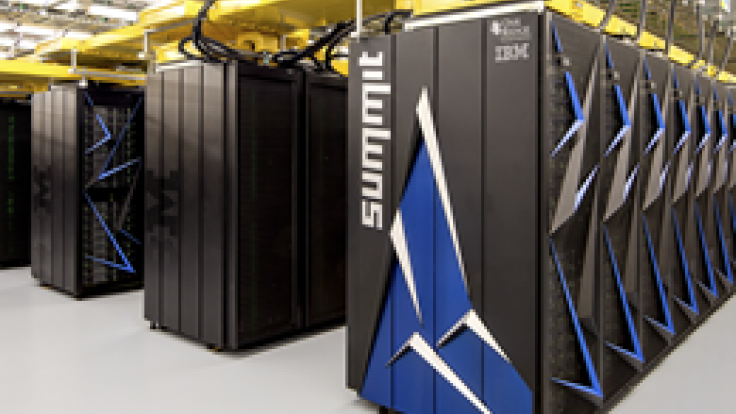
\includegraphics[scale=0.4]{L02_ArchNumbersSystems/L2_summit.png}
            DoE Summit Supercomputer, consisting of 4,608 nodes; 9,216 CPUs; 36,864 cores; 27,648 GPUs; 13 MW for only \$325 million
            \footnotesize
            \url{https://www.olcf.ornl.gov/summit/}
    \end{columns}
    \footnotesize Both run Linux!
\end{frame}

\section{Major Computer Components}
\begin{frame}{Major Computer Components}
    \begin{itemize}
        \item Central Processing Unit (CPU)
        \item Bus
        \item Main memory (RAM)
        \item Secondary storage media
        \item Input/Output (I/O) devices
    \end{itemize}
\end{frame}

\begin{frame}{Schematic Diagram of a Computer}
    \centering
    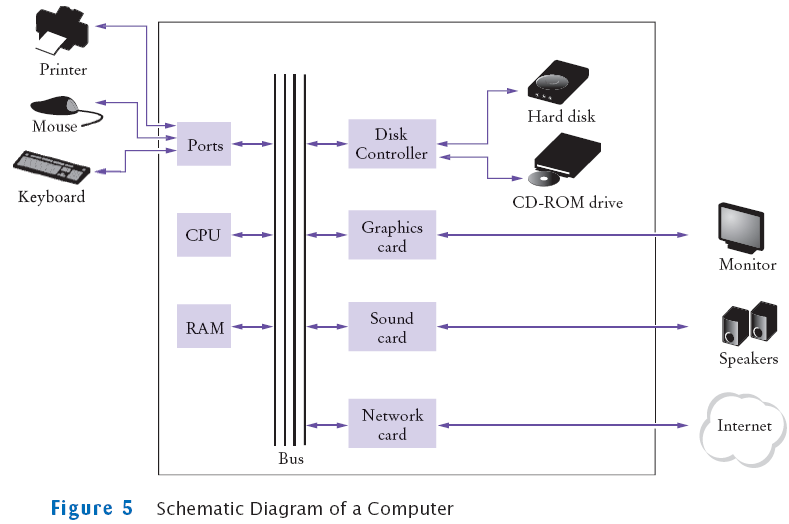
\includegraphics[scale=0.6]{L02_ArchNumbersSystems/L2_p7.png}
    \footnotesize{Diagram taken from Java Concepts, Fourth Edition}
\end{frame}

\begin{frame}{Realistic Diagram of Computer Components}
\centering
    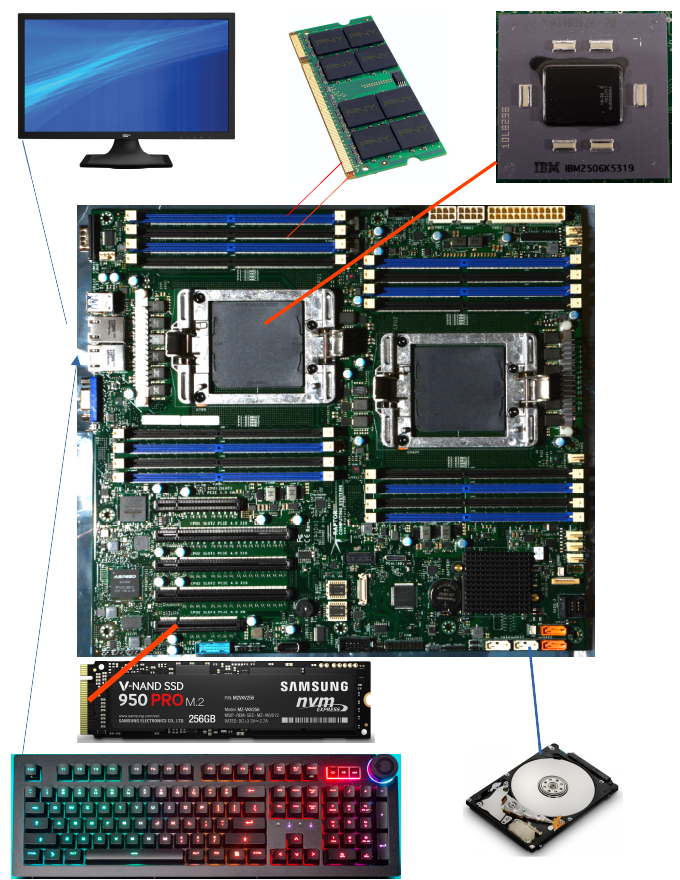
\includegraphics[scale=0.25]{L02_ArchNumbersSystems/L2_p8.png}
\end{frame}

\subsection{CPU}
\begin{frame}{The CPU}
\begin{columns}
    \column{0.6\textwidth}
    \begin{itemize}
        \item Central Processing Unit
        \item The ``brain'' of the computer
        \item Controls all other computer functions
        \item Sometimes called a microprocessor or simply processor
        \item There are different processors for different types of devices (the processor in your computer is very different compared to the processor in your phone)
    \end{itemize}
     \column{0.4\textwidth}
    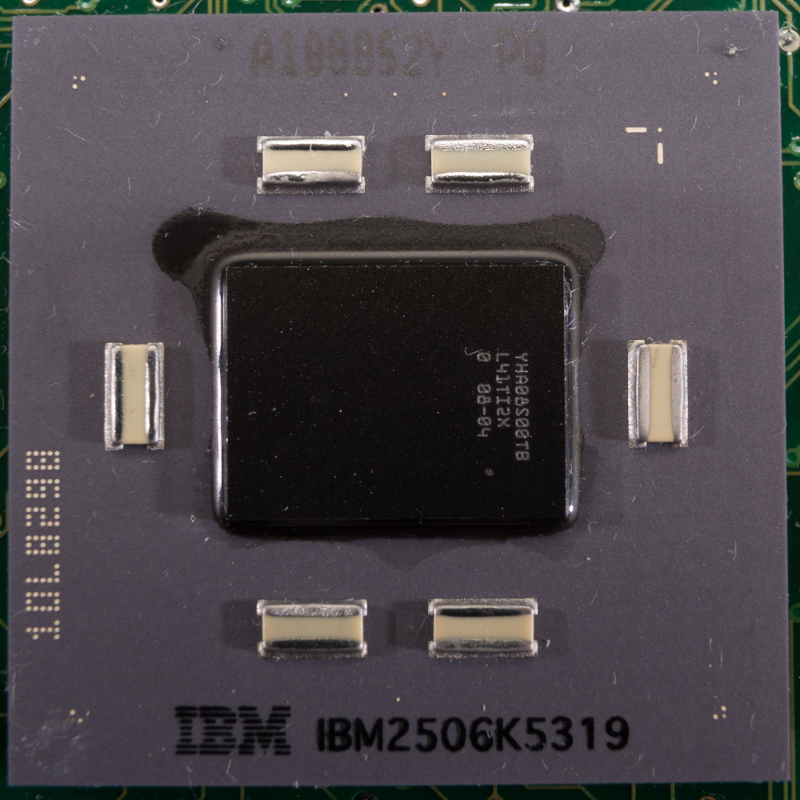
\includegraphics[scale=0.6]{L02_ArchNumbersSystems/L2_p8_cpu.png}
    \end{columns}
\end{frame}

\subsection{Bus}
\begin{frame}{The Bus}
    \begin{itemize}
        \item Computer components are connected by a bus
        \item A bus is a group of parallel wires which carry control signals \& data between components.
        \item Examples:
        \begin{itemize}
            \item PCI = Peripheral Component Interconnect Express\footnote{\url{https://en.wikipedia.org/wiki/PCI_Express}}, connects devices internally, like graphics \& networking cards
            \item USB = Universal Serial \underline{Bus}, connects external devices, like printers, scanners, and many more
            \item Thunderbolt, a mix of the two, allowing typically internal devices to be connected externally
        \end{itemize}
        \item Bluetooth, a wireless protocol, connects accessories to the computer within a short range. It is similar to a bus, but doesn't meet the definition because it's wireless, and typically connects via USB.
    \end{itemize}
\end{frame}

\begin{frame}{The Bus}
    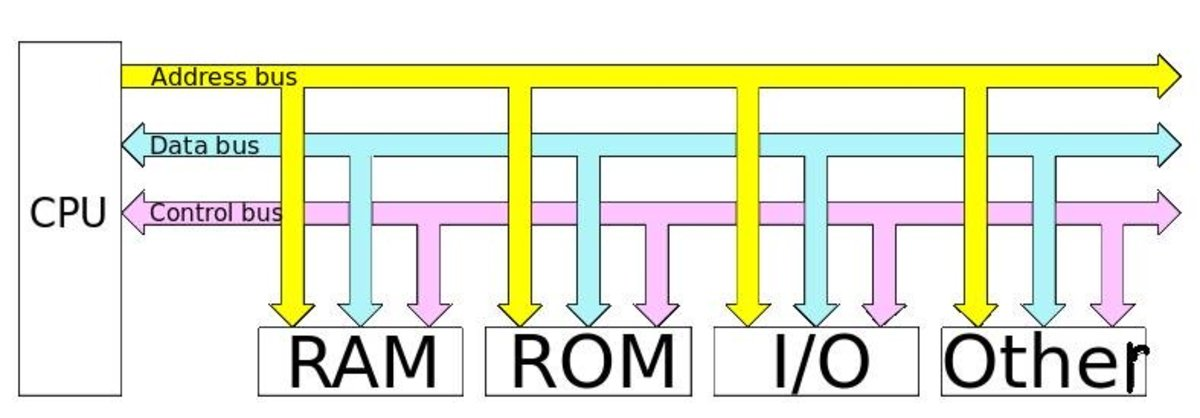
\includegraphics[scale=0.36]{L02_ArchNumbersSystems/L2_buses.jpg}
    \footnotesize{\url{https://upload.wikimedia.org/wikipedia/commons/a/a9/Computer_buses.svg}}
\end{frame}

\subsection{Memory}
\begin{frame}{Main Memory}
\only<1>{
    \begin{columns}
        \column{0.6\textwidth}
        \begin{itemize}
            \item Main memory holds information needed to run the computer, which includes information about the operating system, programs which are running, and everything else which makes the computer usable.
        \end{itemize}
    \column{0.4\textwidth}
        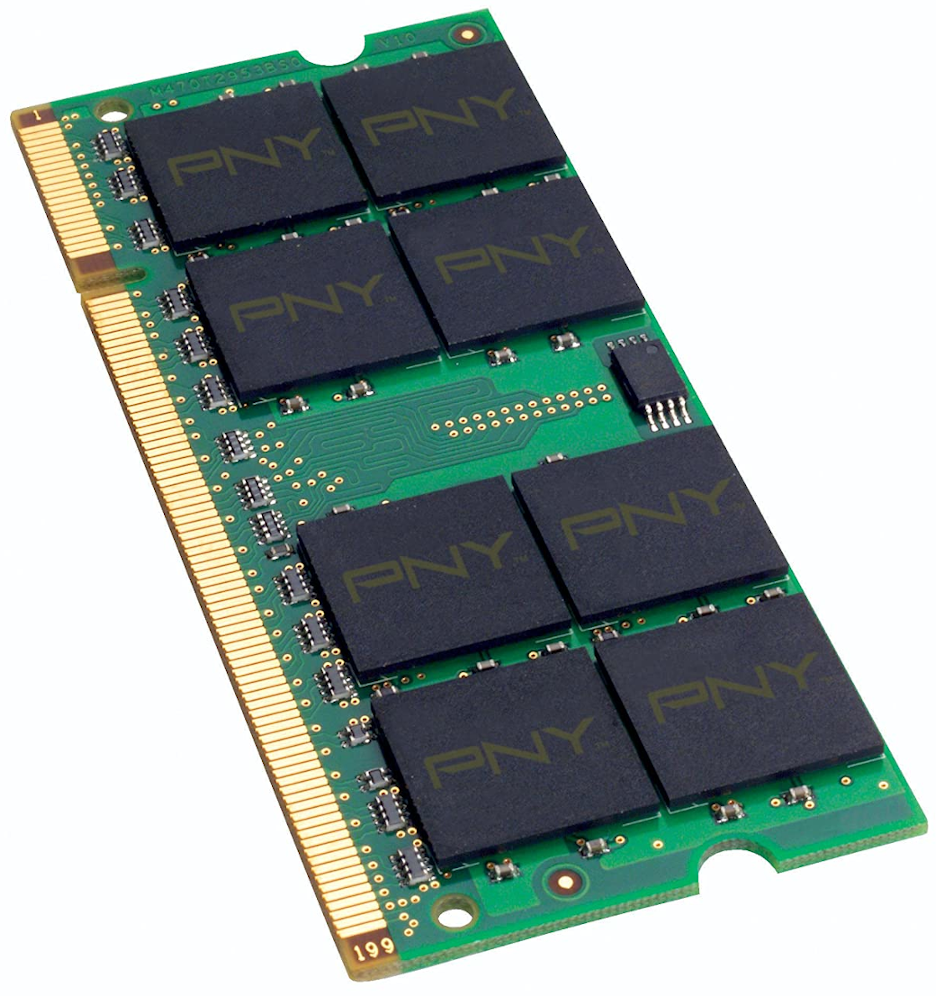
\includegraphics[scale=0.5]{L02_ArchNumbersSystems/L2_p8_ram.png}
    \end{columns}
    }
\only<2> {
    \begin{itemize}
        \item Main memory is made up of transistors.
        \item If the transistor is closed, then it's state is said to be 1, or ON.
        \item If the transistor is open, then it's state is said to be 0, or OFF.
        \item Keeping track of off and on states is why computers use binary numbers.
    \end{itemize}
}
\only<3> {
    \begin{itemize}
        \item Every eight bits is known as a \textit{byte}.
        \item Each of these bytes as uniquely numbered, which is it's \textit{address}.
        \item Memory is volatile storage, meaning that the information is lost when the computer no longer has electricity.
    \end{itemize}
}
\only<4> {
    \begin{itemize}
        \item Other computer components can:
        \begin{itemize}
            \item get the information held at a particular address in memory, known as a \textit{READ},
            \item and store information at a particular address in memory, known as a \textit{WRITE}.
        \end{itemize}
        \item Writing to a memory location alters it's contents, the prior information is lost.
        \item Reading from a memory location does not alter its contents.
        \item Example: when browsing the Internet, the browser sends information to another website.
        \begin{itemize}
            \item The browser writes information to memory
            \item The network card reads the information, sends data across the network
            \item The network card gets information from the server, writes data to memory
            \item The web browser reads the memory and displays it to you.
        \end{itemize}
    \end{itemize}
}
\only<5> {
    \begin{itemize}
        \item All addresses in memory can be accessed in the same amount of time.
        \item The computer doesn't start at address 0 and read until we get to the address we really want (\textit{sequential access}).
        \item The computer goes directly to the address we want and accesses the data (known as \textit{direct} or \textit{random access}).
        \item This is where RAM gets it's name: \textit{Random Access Memory}.
    \end{itemize}
}
\only<6> {
    \begin{itemize}
        \item ``Stupid question'': Why does adding more RAM make the computer faster, or seem faster?
        \item Answer: This is a complicated situation, it has to do with swapping/paging, and multiprocessing.
        \item Portions of memory which aren't used often are saved to the hard drive, to free up memory for programs which are currently running, known as \textit{swapping}. More RAM means more information can be stored at once, and RAM is always faster than the hard drive.
    \end{itemize}
}
\end{frame}

\begin{frame}{Opening MS Word}
    \begin{itemize}
        \item Use the mouse to select MS Word
        \item The CPU requests the MS Word application
        \item MS Word is loaded from the hard drive to main memory
        \item The CPU reads instructions from main memory and executes them one at a time
        \item MS Word appears on your monitor
    \end{itemize}
\end{frame}

\subsection{Storage}
\begin{frame}{Secondary Storage}
    \begin{itemize}
        \item From faster to slower:
        \begin{itemize}
            \item Hard drives (random access)
            \item USB thumb drives (random access)
            \item Optical: CD, DVD, Blu-ray drives (random access)
            \item Floppy drives (random access)
            \item Tapes (sequential access)
        \end{itemize}
        \item These types are known as persistent or permanent storage, since they're non-volatile.
    \end{itemize}
    \begin{columns}
        \column{0.4\textwidth}
            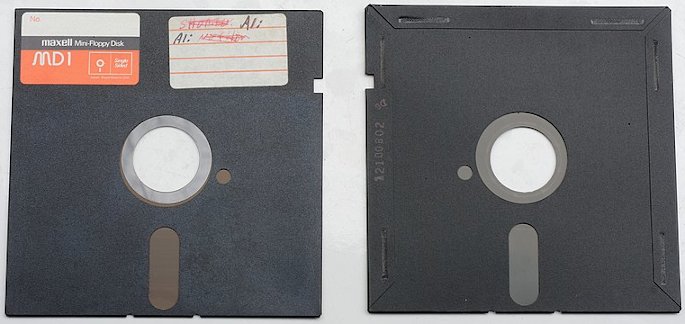
\includegraphics[scale=0.20]{L02_ArchNumbersSystems/L2_p17_525.png}
        \column{0.6\textwidth}
            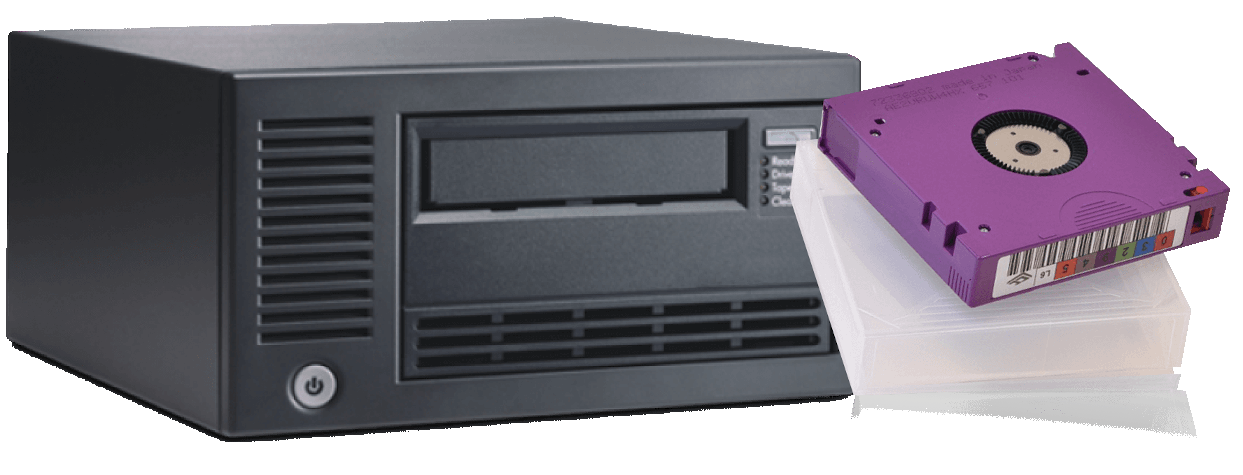
\includegraphics[scale=0.17]{L02_ArchNumbersSystems/L2_p17_tape.png}
    \end{columns}
\end{frame}

\subsection{I/O Devices}
\begin{frame}{Input/Output (I/O) Devices}
    \begin{itemize}
        \item Information input and output is handed by I/O devices, also known as peripheral devices
        \item Examples:
        \begin{itemize}
            \item Monitor (output)
            \item Keyboard (input)
            \item Mouse (input)
            \item Joystick, gamepad (input)
            \item Disk drive (input \& output)
            \item CD-ROM, DVD-ROM (input)
            \item CD, DVD burner (input \& output)
            \item Printer (output)
            \item Scanner (input)
            \item Network card (input \& output)
            \item Sound card (input \& output)
        \end{itemize}
    \end{itemize}
\end{frame}

\section{Bytes, Bits, Words}
\begin{frame}{Bits, Bytes, Words}
    \begin{itemize}
        \item A bit is a single binary digit (zero or one)
        \item A byte is 8 bits
        \item A word is 32 bits, or 4 bytes
        \item Long word = 8 bytes = 64 bits
        \item Quad word = 16 bytes = 128 bits
        \item Programming languages use these standard number of bits when organizing data
    \end{itemize}
\end{frame}

\section{Number Systems}
\begin{frame}{Number Systems}
    \begin{itemize}
        \item The most elementary ``number system'' is unary: ``I have \textit{this} many things''.
        \item An interesting problem: If you had $1+1+1$ things, and you gave away $1+1+1$ of them, how would you answer the question: ``How many do you have left?''
        \item Unary counting is not a symbolic number system.
    \end{itemize}
\end{frame}

\begin{frame}{Unary Numbers Are Not Practical}
    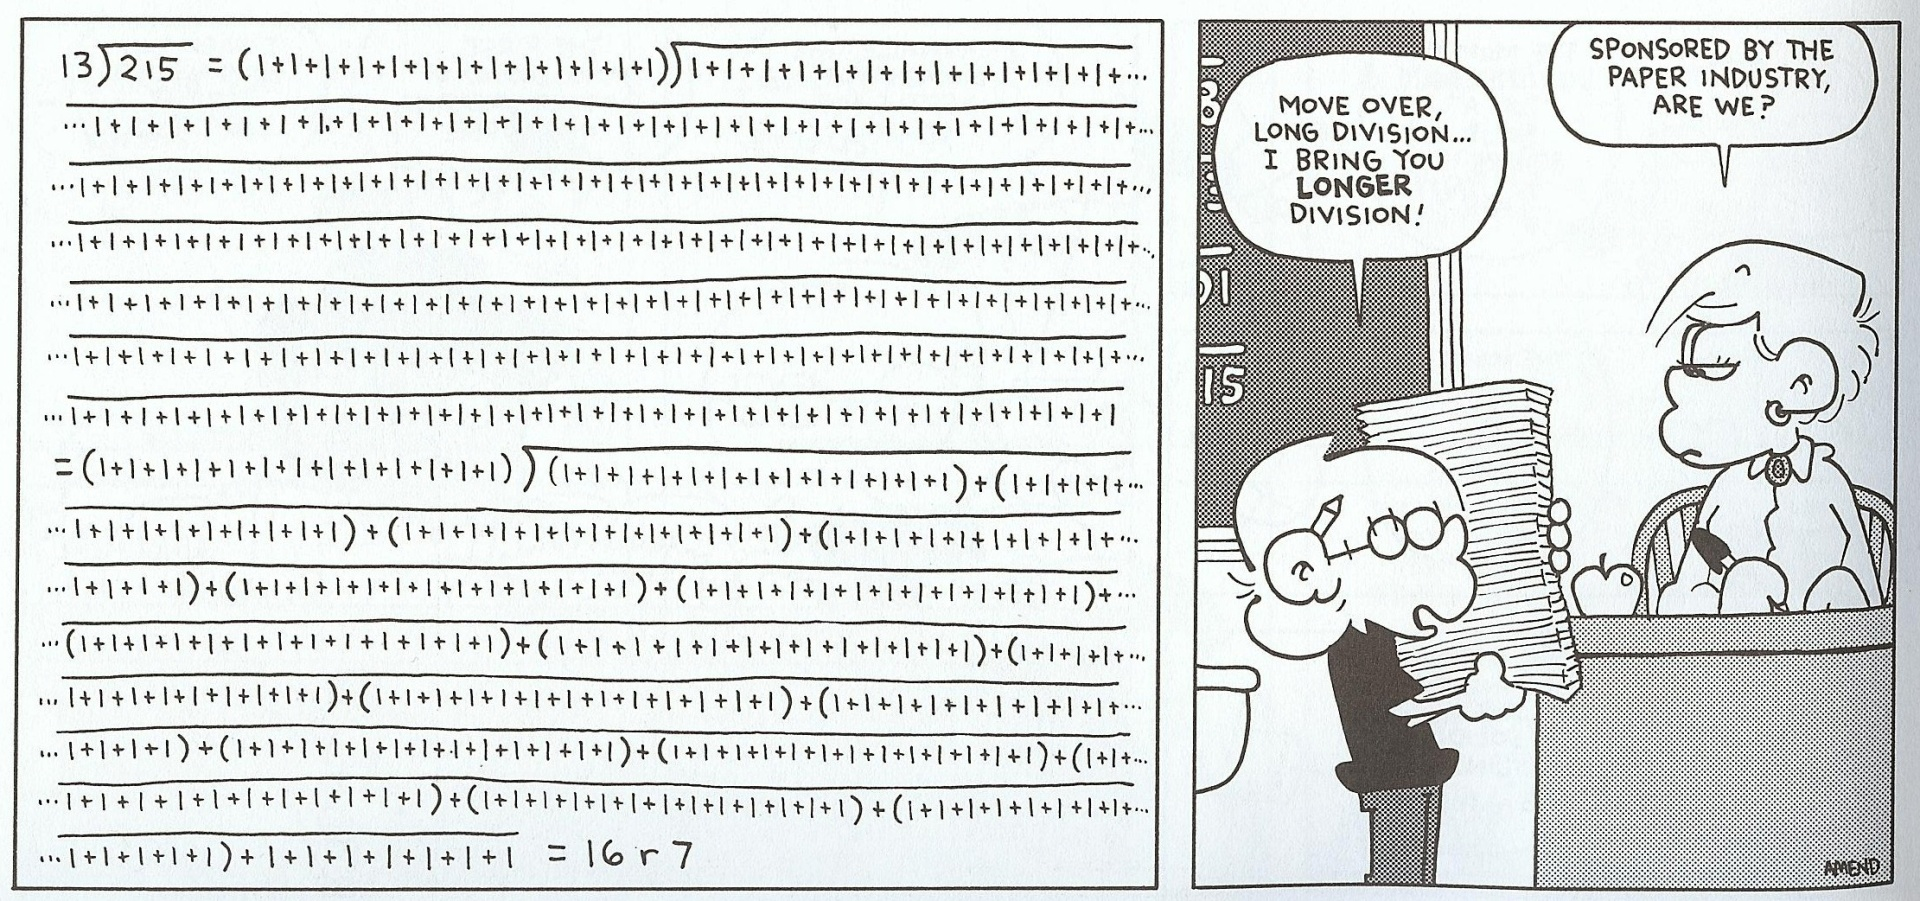
\includegraphics[scale=0.2]{L02_ArchNumbersSystems/L2_p22.png}
\end{frame}

\begin{frame}{Number Systems}
    \begin{itemize}
        \item The on \& off states of the transistors in RAM can be thought of as the values 1 \& 0, respectively.
        \item Therefore, thinking about how information is stored in RAM requires knowledge of the binary (base 2) number system.
        \item Let's review decimal (base 10) first.
    \end{itemize}
\end{frame}

\subsection{Decimal}
\begin{frame}{The Decimal Number System}
    \begin{itemize}
        \item The decimal number system is a positional number system.
    \end{itemize}
    
    \begin{columns}
        \column{0.4\textwidth}
            \begin{tabular}{ c c c c }
                \thead{5} & \thead{6} & \thead{2} & \thead{1} \\ 
                $10^3$ & $10^2$ & $10^1$ & $10^0$
            \end{tabular}
        \column{0.6\textwidth}
            \begin{tabular}{ l l l l l }
                1 & X & $10^0$ & = & 1 \\ 
                2 & X & $10^1$ & = & 20 \\
                6 & X & $10^2$ & = & 600 \\
                5 & X & $10^3$ & = & 5000
            \end{tabular}
    \end{columns}
\end{frame}

\begin{frame}{The Decimal Number System}
    \begin{itemize}
        \item The decimal number system is also known as base 10. The values of the positions are calculated by taking 10 to some power.
        \item Why is the base 10 for decimal numbers?
        \begin{itemize}
            \item Because we use 10 digits, the digits 0 though 9.
        \end{itemize}
        \item The decimal number system, and other number systems, are \textit{symbolic representations} of concrete quantities.
    \end{itemize}
\end{frame}

\subsection{Binary}
\begin{frame}{The Binary Number System}
    \begin{itemize}
        \item The binary number system is also known as base 2. The values of the positions are calculated by taking 2 to some power.
        \item Why is the base 2 for binary numbers?
        \begin{itemize}
            \item Because we use 2 digits, the digits 0 and 1.
            \item Because the underlying circuit is either off or on; or open or closed. There's no other state.
        \end{itemize}
    \end{itemize}
\end{frame}

\begin{frame}{The Binary Number System}
    \begin{itemize}
        \item The binary number system is also a positional number system.
        \item Instead of using ten digits, $0\rightarrow9$, the binary system uses only two digits, 0 and 1.
        \item Example, going back to the number 5621 from the decimal example:
    \end{itemize}
    \\ ~~ \\
    \begin{tabular}{ l l l l l l l l l l l l l }
        \thead{1} & \thead{0} & \thead{1} & \thead{0} & \thead{1} & \thead{1} & \thead{1} & \thead{1} & \thead{1} & \thead{0} & \thead{1} & \thead{0} & \thead{1} \\
        $2^{12}$ & $2^{11}$ & $2^{10}$ & $2^9$ & $2^8$ & $2^7$ & $2^6$ & $2^5$ & $2^4$ & $2^3$ & $2^2$ & $2^1$ & $2^0$ \\
        4096 & & 1024 & & 256 & 128 & 64 & 32 & 16 & & 4 & 1
    \end{tabular}
\end{frame}

\subsection{Binary to Decimal}
\begin{frame}{Converting from Binary to Decimal}
    \begin{columns}
        \column{0.6\textwidth}
            \begin{tabular}{l l l l l l l l}
                 \thead{0} & \thead{1} & \thead{0} & \thead{0} & \thead{1} & \thead{1} & \thead{0} & \thead{1} \\
                 $2^7$ & $2^6$ & $2^5$ & $2^4$ & $2^3$ & $2^2$ & $2^1$ & $2^0$\tikz[remember picture] \node[coordinate,anchor=west] (n1) {};
            \end{tabular}
            \\ ~~ \\
            \begin{tabular}{| l l |}
                \hline
                $2^0=1$ & $2^4=16$  \\
                $2^1=2$ & $2^5=32$  \\
                $2^2=4$ & $2^6=64$  \\
                $2^3=8$ & $2^7=128$ \\
                \hline
            \end{tabular}
        \column{0.4\textwidth}
            \begin{tabular}{r r}
                 \tikz[baseline, remember picture] \node[anchor=west] (t1){};$1X2^0$ & 1 \\
                 $0X2^1$ & 0 \\
                 $1X2^2$ & 4 \\
                 $1X2^3$ & 8 \\
                 $0X2^4$ & 0 \\
                 $0X2^5$ & 0 \\
                 $1X2^6$ & 64 \\
                 $0X2^7$ & 0 \\
                 \hline\hline
                 & $77_{10}$
            \end{tabular}
    \end{columns}
    \begin{tikzpicture}[remember picture,overlay]   %% use here too
        \path[draw=red,thin,->] -- ([xshift=1mm] n1.west) to (t1.west);
    \end{tikzpicture}
\end{frame}

\begin{frame}{Converting from Binary to Decimal}
    \begin{itemize}
        \item Practice conversions:
    \end{itemize}
    \centering
    \only<1> {
        \begin{tabular}{r r}
            \thead{Binary} & \thead{Decimal} \\
             11101 & \\
             1010101 & \\
             100111 & \\
             10010110 &
        \end{tabular}
    }
    \only<2> {
        \begin{tabular}{r r}
            \thead{Binary} & \thead{Decimal} \\
             11101 & 29 \\
             1010101 & \\
             100111 & \\
             10010110 &
        \end{tabular}
    }
    \only<3> {
        \begin{tabular}{r r}
            \thead{Binary} & \thead{Decimal} \\
             11101 & 29 \\
             1010101 & 85 \\
             100111 & \\
             10010110 &
        \end{tabular}
    }
    \only<4> {
        \begin{tabular}{r r}
            \thead{Binary} & \thead{Decimal} \\
             11101 & 29 \\
             1010101 & 85 \\
             100111 & 39 \\
             10010110 &
        \end{tabular}
    }
    \only<5> {
        \begin{tabular}{r r}
            \thead{Binary} & \thead{Decimal} \\
             11101 & 29 \\
             1010101 & 85 \\
             100111 & 39 \\
             10010110 & 150
        \end{tabular}
    }
\end{frame}

\begin{frame}{Geek Joke \#1}
    \begin{itemize}
        \item Seen on a T-shirt:
    \end{itemize}
    There are 10 kinds of people in the world: Those who understand binary, and those who don't.
\end{frame}

\begin{frame}{Converting from Decimal to Binary}
    \begin{itemize}
        \item Make a list of the binary place values up to the number being converted.
        \item Perform successive divisions by 2, placing the remainder of 0 or 1 in each of the positions from right to left.
        \item Continue until the quotient is zero.
        \item Example: $42_{10}$
    \end{itemize}
    \\ ~~ \\
    \centering
    \begin{tabular}{c l l l l l l}
        \redout{\thead{64}} & \thead{32} & \thead{16} & \thead{8} & \thead{4} & \thead{2} & \thead{1} \\
        & 1 & 0 & 1 & 0 & 1 & 0 \\
        \redout{$2^6$} & $2^5$ & $2^4$ & $2^3$ & $2^2$ & $2^1$ & $2^0$
    \end{tabular}
\end{frame}

\subsection{Decimal to Binary}
\begin{frame}{Converting from Decimal to Binary}
    \begin{itemize}
        \item Practice conversions:
    \end{itemize}
    \centering
    \only<1> {
        \begin{tabular}{r r}
            \thead{Decimal} & \thead{Binary} \\
             59  & \\
             82  & \\
             137 & \\
             175 &
        \end{tabular}
    }
    \only<2> {
        \begin{tabular}{r r}
            \thead{Decimal} & \thead{Binary} \\
             59  & 111011 \\
             82  & \\
             137 & \\
             175 &
        \end{tabular}
    }
    \only<3> {
        \begin{tabular}{r r}
            \thead{Decimal} & \thead{Binary} \\
             59  & 111011 \\
             82  & 1010010 \\
             137 & \\
             175 &
        \end{tabular}
    }
    \only<4> {
        \begin{tabular}{r r}
            \thead{Decimal} & \thead{Binary} \\
             59  & 111011 \\
             82  & 1010010 \\
             137 & 10001001 \\
             175 &
        \end{tabular}
    }
    \only<5> {
        \begin{tabular}{r r}
            \thead{Decimal} & \thead{Binary} \\
             59  & 111011 \\
             82  & 1010010 \\
             137 & 10001001 \\
             175 & 10101111
        \end{tabular}
    }
\end{frame}

\begin{frame}{Working with Large Numbers}
    0 1 0 1 0 0 0 0 1 0 1 0 0 1 1 1 = ?
    \\ ~~ \\
    \begin{itemize}
        \item Humans can't work well with binary numbers, there are too many digits!
        \item Memory addresses, and other data, can be quite large. Therefore, we sometimes use the hexadecimal (base 16) and octal (base 8) number systems.
    \end{itemize}
\end{frame}

\subsection{Hexadecimal}
\begin{frame}{The Hexadecimal Number System}
    \only<1> {
        \begin{itemize}
            \item The hexadecimal number system is also known as base 16. The values of the positions are calculated by taking 16 to some power.
            \item What is it base 16 for hexadecimal numbers?
            \begin{itemize}
                \item Because we use 16 symbols, the digits 0 through 9, and the letters A through F.
            \end{itemize}
        \end{itemize}
    }
    \only<2> {
        \begin{tabular}{r c c | r c c}
             \thead{Binary} & \thead{Decimal} & \thead{Hexadecimal} & \thead{Binary} & \thead{Decimal} & \thead{Hexadecimal}  \\
             0    & 0 & 0 & 1010 & 10 & A \\
             1    & 1 & 1 & 1011 & 11 & B \\
             10   & 2 & 2 & 1100 & 12 & C \\
             11   & 3 & 3 & 1101 & 13 & D \\
             100  & 4 & 4 & 1110 & 14 & E \\
             101  & 5 & 5 & 1111 & 15 & F \\
             110  & 6 & 6 & 10000 & 16 & 10 \\
             111  & 7 & 7 & 10001 & 17 & 11 \\
             1000 & 8 & 8 &       &    & \\
             1001 & 9 & 9 & 11011 & 27 & 1B
        \end{tabular}
    }
    \only<3> {
        \begin{itemize}
            \item Example of a hexadecimal number and the values of the positions:
        \end{itemize}
        \\ ~~ \\
        \begin{tabular}{c c c c c c c c}
             \thead{3} & \thead{C} & \thead{8} & \thead{B} & \thead{0} & \thead{5} & \thead{1} & $\rightarrow63483985$ \\
             $16^6$ & $16^5$ & $16^4$ & $16^3$ & $16^2$ & $16^1$ & $16^0$ & 
        \end{tabular}
    }
\end{frame}

\subsection{Octal}
\begin{frame}{The Octal Number System}
    \begin{itemize}
        \item Example of an octal number and the values of the positions:
    \end{itemize}
    \\ ~~ \\
    \center{
        \begin{tabular}{c c c c c c}
             \thead{1} & \thead{3} & \thead{0} & \thead{0} & \thead{2} & \thead{4} \\
             $8^5$ & $8^4$ & $8^3$ & $8^2$ & $8^1$ & $8^0$ 
        \end{tabular}
    }
    \begin{itemize}
        \item Binary equivalent:
        \begin{itemize}
            \item 1 011 000 000 010 100 $\rightarrow$ 1011000000010100
        \end{itemize}
    \end{itemize}
\end{frame}

\begin{frame}{Example of Equivalent Numbers}
    \begin{tabular}{l l}
         Binary:      & 1 1 0 1 0 0 0 0 1 0 1 0 0 1 1 1  \\
         Octal:       & $150247_8$ (or O150247) \\
         Decimal:     & $53414_{10}$ \\
         Hexadecimal: & $D0A7_{16}$ (or 0xD0A7, or D0A7h)
    \end{tabular}
    \\ ~~ \\ ~~ \\
    Notice that the number of digits decreases as the the base increases.
\end{frame}

\begin{frame}{Why Use Hexadecimal or Octal?}
    \begin{itemize}
        \item Use fewer characters
        \item Can easily convert between non-decimal numbers
        \begin{itemize}
            \item Divide numbers into equal-sized sets of bits, then convert directly
            \item \textit{Not} true of decimal to binary, hex, or octal
        \end{itemize}
    \end{itemize}
\end{frame}

\end{document}